\documentclass[11pt]{article}
\usepackage[margin=1in]{geometry}
\usepackage{hyperref}
\usepackage{graphicx}
\usepackage{amsmath}
\usepackage{enumitem}
\usepackage{listings}
\usepackage{xcolor}
\usepackage{draftwatermark}
\SetWatermarkText{DRAFT}
\SetWatermarkScale{3}
\SetWatermarkColor[gray]{0.85}

\definecolor{lightgray}{gray}{0.95}
\lstset{
  basicstyle=\ttfamily\small,
  backgroundcolor=\color{lightgray},
  breaklines=true,
  columns=fullflexible
}

\title{IPv6-Only HTCondor Integration with the Open Science Pool: \\
The Viper Cluster at GW/CAAREN}
\author{Research Technology Services, GWIT\\
The George Washington University}
\date{\today}

\begin{document}

\maketitle

\begin{abstract}
This paper presents the successful integration of a single-stack IPv6 HTCondor cluster into the Open Science Pool (OSPool) by The George Washington University in partnership with the Capital Area Advanced Research and Education Network (CAAREN). 
Designed to operate entirely within an IPv6-only environment, this demonstrates the feasibility of contributing 
high-throughput computing resources to the OSPool without legacy IPv4 support. We address key challenges in ensuring compatibility
with both OSPool and HTCondor in addition to heterogeneous user workloads, many of which assume IPv4 availability. By leveraging
connection brokering (CCB), NAT64/CLAT translation, and robust IPv6 network services, this deployment serves as a model for institutions
planning for IPv6-only infrastructure while maintaining full interoperability with national research computing platforms.
\end{abstract}
\tableofcontents

\section{Introduction}

The George Washington University~\cite{gwu}, in partnership with the Capital Area Advanced Research and Education Network (CAAREN)~\cite{caaren},  
\href{https://ce-dashboard.ospool.osg-htc.org/overview.html?host=gwu-viper-ce1&r=week}{successfully} 
contributed a single-stack IPv6 HTCondor~\cite{htcondor} cluster, Viper, to the Open Science Pool (OSPool)~\cite{ospool}, a nationally distributed computing platform for data-intensive research.~\cite{pordes2007,sfiligoi2009,osgospool,osgfs} This demonstrates a path forward for institutions preparing for an IPv6-only future, reinforcing GW’s leadership in research cyberinfrastructure and open science.

There is some legitimate concern that integrating IPv6-only computational resources into the OSPool may have adverse effects on effective job throughput. These concerns break down into two broad categories of challenges, 
\begin{enumerate}[itemsep=1pt]
\item IPv6-only interoperability with OSPool and HTCondor 
\item IPv6-only interoperability with researcher jobs which depend on legacy IP. 
\end{enumerate}

A solution is required that bridges the gap for both of these sets of concerns for there to be any possibility of moving beyond legacy addressing. Because the way the OSPool CE's match requests with resources is well-understood~\cite{ospooldocs}, the first set of challenges may be addressed systematically. However, the second set, owing to researcher workflows being much less predictable, requires a broadly-scoped solution that handles a variety of scenarios. 

In this paper we discuss the process of configuring an IPv6-only compute resource for integration into the OSPool.

\section{System Overview}

Viper is a 12-node HTCondor cluster managed with Warewulf 4.6.1~\cite{warewulf} running Rocky Linux 9.5 and supported by a dedicated network-attached ZFS pool for backups and administrative workflows.  Each node in the cluster is a Dell PowerEdge R730 with the following hardware specifications:

\begin{center}
\small
\begin{tabular}{|l|l|}
\hline
\textbf{Component} & \textbf{Specification} \\
\hline
Cores & 2x14 Intel Xeon E5-2680 v4 @ 2.40GHz\\
RAM & 8x16 GB DIMM ECC 2400 MT/s \\
Scratch Storage & 1 TB SSD \\
\hline
\end{tabular}
\end{center}
There  are two master nodes serving as redundant central-managers in an active-passive relation, one
submit node, and nine execute points. Because Viper uses Warewulf's stateless provisioning, nodes can be quickly repurposed or recovered after failure.

Viper is configured to advertise 4.5 GB of RAM per core to the Open Science Pool, allowing it to efficiently integrate with workloads of varying shapes.  

\section{About CAAREN}

The Capital Area Advanced Research and Education Network (CAAREN) provides high-performance networking to support education, research, and innovation in the Washington, D.C. area. As a regional optical network and member of Internet2, CAAREN connects GW to other research institutions and to global science collaborations.
\newline

CAAREN has been a leader in routing security, being among the first US higher education institutions to implement Route Origin Authorization (ROAs).  CAAREN implemented the first know production deployment of TCP-AO for advanced BGP session security~\cite{TCPAO}.
\newline

Also available on CAAREN is an advanced content distribution test environment using Tree Distribution Networking (TreeDN)~\cite{TreeDN}.  Employing a combination of native multicast and overlay tunneling technology (via Automatic Multicast Tunneling - AMT), multicast content can be delivered to any endpoint.
\newline

CAAREN’s core network includes:
\begin{itemize}[leftmargin=*,itemsep=1pt]
 \item Juniper MX480 
\item DWDM with optical protection to connect to Intenet2
 \item Supplemental 10 Gbps access via secondary switches
\end{itemize}

Additional CAAREN services include:
\begin{itemize}[leftmargin=*,label=–,itemsep=1pt]
 \item Cloud Connect: Dedicated links via Internet2’s footprint to AWS, Azure, Google Cloud, and OCI, offering low-latency, secure access to cloud resources.
 \item The Things Network: A collaborative IoT sensor network initiative using LoRaWAN for low-power, long-range device communication.
\end{itemize}

These services position CAAREN as a leader for data-intensive science, advanced networking research, and the transition to secure, scalable IPv6-only architectures.

\section{About The OSPool}
The Open Science Pool (OSPool), organized by the Open Science Grid (OSG) consortium, provides access to a large-scale, distributed high throughput computing (HTC) fabric that supports research across a wide range of scientific domains in the United States~\cite{ospool}. Resources in the OSPool are contributed by over 100 partner institutions—including universities, national laboratories, and research centers—and coordinated through a shared infrastructure designed for scalable and opportunistic use.

In the past year alone, OSPool delivered over 1.2 billion CPU hours to U.S. researchers, enabling elastic compute capability through its “submit locally, run globally” model. Researchers can submit jobs from their home institution or an OSG-managed access point and expand into the broader pool when local capacity is exceeded~\cite{ospoolutil}.


\subsection{Compute Entrypoints and Glidein Jobs}
To support this ecosystem, the OSG provides a complete, integrated software stack for job submission, resource provisioning, and monitoring. Sites that contribute resources run compute and storage services using this stack expose capacity through HTCondor-based interfaces such as OSG Compute Entrypoints (CEs). The OSPool architecture is designed to interoperate across heterogeneous environments, including support for emerging network models such as IPv6-only deployments.

In the Open Science Pool (OSPool), Compute Entrypoints (CEs) serve as the gateway for job submissions into local resources such as Viper. Instead of receiving  user jobs directly, CEs admit pilot jobs—called {\it glideins} which are launched by a central pilot factory. Each glidein allocates local cluster resources and creates a beachhead from which it runs a bundled HTCondor instance, forming a temporary node within a larger distributed HTCondor pool. These pilots request user jobs from OSPool access points and execute them within a controlled wrapper environment which may include Singularity or Apptainer containers for workload isolation.~\cite{htcondor,glideinwms}

A glidein carries its own lightweight HTCondor configuration and daemons (typically condor\_startd and condor\_master), enabling it to operate independently of the host's local HTCondor setup. During startup, the glidein registers with one or more central managers (collectors) and advertises itself as an available resource. Once matched with a user job, it supervises execution, reports status, and eventually retires after serving its purpose.

To support IPv6-only or NAT'd environments, HTCondor employs the Condor Connection Broker (CCB).~\cite{ccbdesign} CCB allows the pilot to initiate a persistent outbound connection to a central collector which also acts as a CCB server, enabling reverse communication for job dispatch and control. The OSPool's highly available collectors, hosted at institutions like the University of Wisconsin and University of Chicago, broker these connections and provide load balancing and fault tolerance.

%\section{OSPool IPv6-Only Integration}


\section{Network Architecture}

Viper is integrated into the CAAREN research network using globally routable IPv6 addresses on all nodes. IPv6 is the sole transport protocol used for all HTCondor daemons and management tools. Figure~\ref{fig:viper-network} illustrates the overall layout and connectivity of the Viper deployment.

\subsection{IPv6 Addressing and Interface Layout}

Each node has a statically assigned IPv6 address from a globally routable /64 prefix delegated to GWU by CAAREN. The interface layout is as follows:
\begin{itemize}[leftmargin=*,label=--,itemsep=1pt]
    \item \textbf{Primary interface:} \texttt{eno1}, used for HTCondor daemon communication and OSPool job I/O
    \item \textbf{Secondary interface:} \texttt{clat0}, a virtual interface created by CLATD to support legacy IPv4-only applications using 464XLAT translation
\end{itemize}

No IPv4 addresses are assigned to any interface on the system, and all name resolution, routing, and job submission are performed over IPv6.

\subsection{Routing and Firewalling}

Routing within Viper and upstream to the internet is handled via CAAREN’s core routers. Internally, the cluster uses host-based firewalls to limit inbound IPv6 traffic. The following constraints are enforced:
\begin{itemize}[leftmargin=*,label=--,itemsep=1pt]
    \item Inbound traffic from specific OSG ranges is allowed for HTCondor job and daemon communication
    \item Outbound traffic is unrestricted to allow for software installation, data transfer, and job staging
    \item ICMPv6 and multicast traffic necessary for neighbor discovery are explicitly allowed
\end{itemize}

There are no intermediate firewalls or NAT devices on the local network path. All firewall rules are managed and deployed via the stateless overlay system to ensure consistency across nodes.

\subsection{DNS64/NAT64 Infrastructure}

To support outbound connections to IPv4-only resources (e.g., public repositories or APIs), the cluster relies on:
\begin{itemize}[leftmargin=*,label=--,itemsep=1pt]
    \item \textbf{DNS64 resolvers:} Provided via systemd-resolved on the submit node and propagated to all compute nodes
    \item \textbf{NAT64 gateway:} An external, stateless NAT64 service provided by CAAREN’s upstream connectivity 
\end{itemize}

This infrastructure allows IPv6-only nodes to resolve and connect to IPv4 services without needing dual-stack configurations. See Section~\ref{sec:dns-nat}.

\subsection{464XLAT Translation Path}

Each node runs a local instance of \texttt{clatd}, which invokes stateless NAT64 translation to handle IPv4-bound traffic. This includes glideins, containers, and researcher data that depend on IPv4. See Section~\ref{sec:clatd}.



\begin{figure}[htbp]
  \centering
  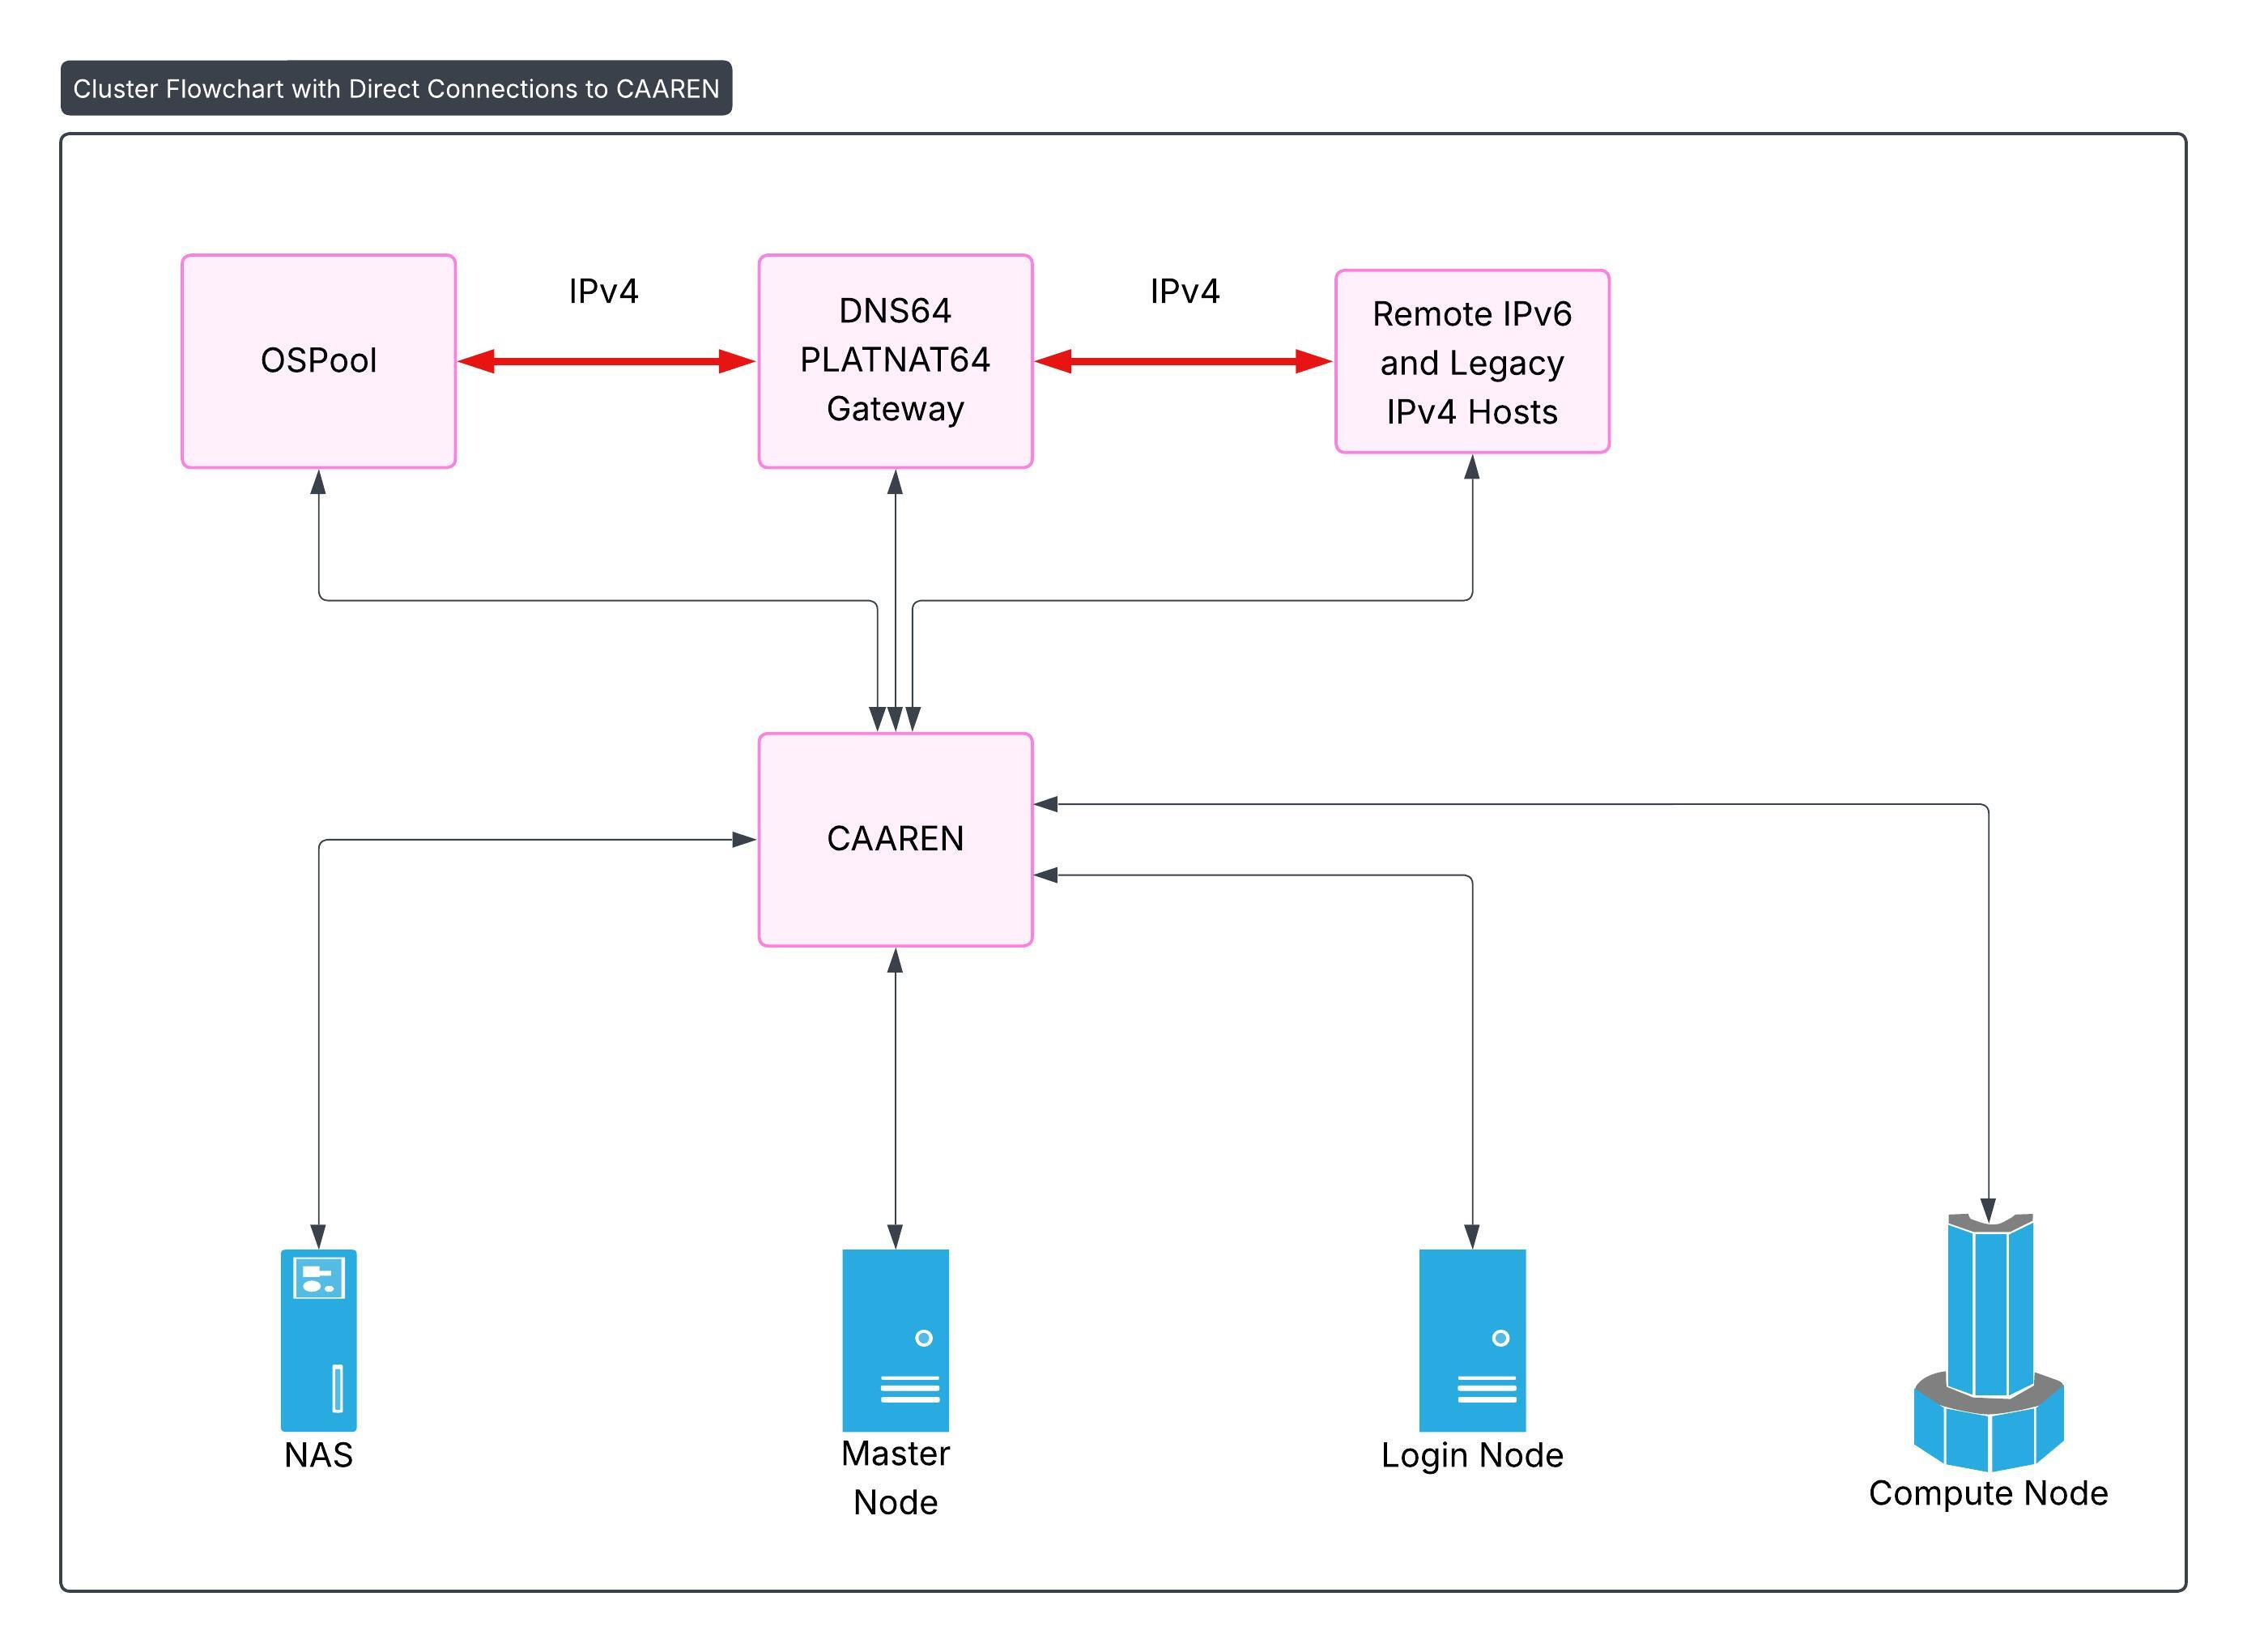
\includegraphics[width=0.49\linewidth]{Viper_Network.jpeg}
  \caption{Network overview of the Viper IPv6-only implementation.}
  \label{fig:viper-network}
\end{figure}


\section{HTCondor Configuration and IPv6 Deployment}
Network configuration is thoroughly discussed in the HTCondor documentation~\cite{htcondor-ipv6}. All HTCondor components are configured to operate only over IPv6. The following key values were set on each node via overlay.

\subsection{Access Point and Central-Manager IPs}
Note that the addresses below are reserved for documentation and used for illustrative purposes; they will need to be updated for site-specific networks.  
\begin{center}
\small
\begin{tabular}{|l|l|}
\hline
\textbf{Role} & \textbf{IPv6 Address} \\
\hline
Central-Manager (CONDOR\_HOST) & \texttt{2001:db8:0:1::200} \\
Submit/Access Point & \texttt{2001:db8:0:1::100} \\
\hline
\end{tabular}
\end{center}

\subsection{/etc/condor/config.d/10\_ipv6.conf}
\begin{lstlisting}[caption={IPv6 Override Settings}, label={lst:ipv6-conf}]
# submit/access point
UID_DOMAIN = 2001:db8:0:1::100

# central-manager
CONDOR_HOST = 2001:db8:0:1::200
COLLECTOR_HOST = [2001:db8:0:1::200]:9618

NETWORK_INTERFACE = eno1
ENABLE_IPV6 = true
PREFER_IPV6 = true
ENABLE_IPV4 = false

ALLOW_READ = 2001:db8:0:1::/64
ALLOW_WRITE = 2001:db8:0:1::/64
ALLOW_NEGOTIATOR = 2001:db8:0:1::/64
ALLOW_ADVERTISE_STARTD = 2001:db8:0:1::/64
\end{lstlisting}

By default, HTCondor sets \texttt{BIND\_ALL\_INTERFACES = true}. In a multi-interface environment, each with network routes, it may be necessary to be more selective. As each execute point on Viper has two interfaces (one being the virtual \texttt{clat} interface), routing tables are used to sidestep this issue. All IPv6 traffic between Condor daemons is bound to the appropriate interface.  


\section{DNS64, NAT64, and 464XLAT}

Viper operates in an IPv6-only environment so some measures are required to enable connectivity to legacy IPv4 hosts and applications. This is achieved through a combination of DNS64, NAT64, and CLAT, an implementation of 464XLAT~\cite{464xlat}.

DNS64 and NAT64 are required for accessing upstream OSG services, Git repositories, and software mirrors that remain IPv4-only.
\subsection{DNS64 and NAT64}
\label{sec:dns-nat}
\begin{itemize}[leftmargin=*,label=--,itemsep=1pt]
  \item \textbf{DNS64:} When an IPv6-only host makes a DNS request for an A record (IPv4), a DNS64-enabled resolver synthesizes an AAAA record using a configured NAT64 prefix, often \texttt{64:ff9b::/96}, but in the case of Viper an external NAT64 gateway was used.
  \item \textbf{NAT64:} The NAT64 gateway intercepts IPv6 packets destined for these synthesized addresses and translates them to the corresponding IPv4 address, enabling IPv4 interoperability.
\end{itemize}


  
\subsection{CLAT for Application Compatibility}
\label{sec:clatd}
Some applications do not support IPv6,  including those that bind to literal,  or hardcoded IPv4 addresses. To address this limitation, Viper utilizes the following:

\begin{itemize}[leftmargin=*,label=--,itemsep=1pt]
  \item \textbf{CLAT (Customer-side Translator):} An open source implementation \cite{clatd} of 464XLAT~\cite{464xlat}, \texttt{CLATD} allows IPv4-only applications to operate in Viper's  IPv6-only environment.  \texttt{CLATD} orchestrates the translation of IPv4 socket calls into IPv6, which are then handled by Viper’s provider-side translator (PLAT)—the NAT64 gateway responsible for bridging to legacy IPv4 services.
  \item \textbf{Implementation:} On Viper, \texttt{CLATD} runs on each node and provides its own instance of \texttt{TAYGA}, an out-of-kernel stateless NAT64 daemon. \texttt{CLATD} (and \texttt{TAYGA}) are integrated at boot through systemd units within overlays. 
\end{itemize}

Note, in a dual-stack environment (e.g., while transitioning from legacy to IPv6) it is important that HTCondor not attempt to bind to the virtual \texttt{clat} interface for intra-daemon communication. It is typically sufficient to specify the appropriate interface by setting \texttt{NETWORK\_INTERFACE} and redirecting all other IPv4-bound traffic to the \texttt{clat} interface.  


Together, DNS64, NAT64, and CLAT allow IPv6-only nodes to maintain operational capability with legacy IP hosts and applications. 

\section{Results and Discussion}

\begin{figure}[htbp]
  \centering
  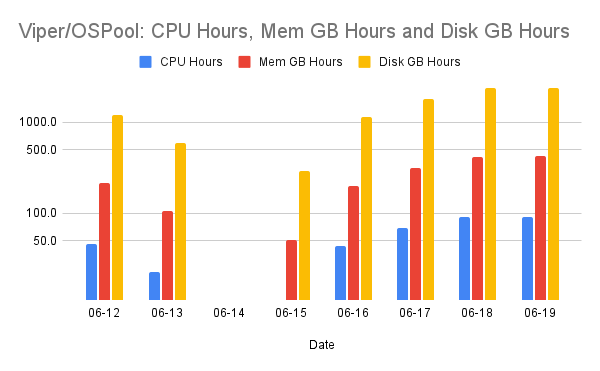
\includegraphics[width=0.49\linewidth]{Viper_OSPool_utilization.png}
  \caption{PLACEHOLDER -- Eight days of processing jobs for the OSPool.}
  \label{fig:viper-jobs}
\end{figure}


\begin{itemize}
\item Viper has been integrated successfully into the OSPool. See Figure~\ref{fig:viper-jobs}. 
\item Despite signaling ENABLE\_IPV4 = false and PREFER\_IPv6 = true.
%\item Glidein jobs are using IPv6 connect to AWS. 
\item Glidein jobs using IPv4 to connect to redundant CCB's (U. Wisconsin and U. Chicago).
\end{itemize}

\subsection{Legacy Support with 464XLAT}

On Viper, each execute point runs a lightweight CLAT daemon, which provides IPv4 compatibility without assigning the node a routable IPv4 address. HTCondor daemons and job payloads bind locally to the IPv4 loopback address 192.0.0.1, satisfying legacy expectations within the software stack. Would-be outbound legacy IPv4 connections are translated through the NAT64 gateway, removing the need for private or public IPv4 space. With DNS64 synthesizing IPv6 addresses for A-records and NAT64 translating at the network boundary, most IPv4-only services become reachable from the IPv6-only environment and, in the event of legacy IP literals, \texttt{clatd} provides the necessary IPv6 translation. 

\subsection{Role of the Condor Connection Broker (CCB)}

In traditional IPv4 NAT or firewall-restricted environments, inbound connections to pilots are blocked, and HTCondor relies on the Condor Connection Broker (CCB) to reverse the communication flow; each glidein opens an outbound connection to a central CCB-enabled collector, which serves as a coordination point for job control and matchmaking.

Glideins deployed by OSPool appear to default to using CCB. In Viper’s case, however, the execute points have publicly routable IPv6 addresses so direct connections from the OSPool are allowed. As such, CCB is not the only viable communication path, but it remains the default for OSG glideins. As more sites with single-stack IPv6 are integrated into the OSPool, it may be worthwile to reconsider relaxing the glidein's CCB dependency.

\subsection{Avoiding Configuration Pitfalls}

Although HTCondor supports IPv6-only operation, legacy components may still expect an IPv4 address. Rather than enabling full dual-stack, Viper configures a non-routable IPv4 loopback alias, via CLAT. This ensures compliance with any IP literals while keeping external traffic strictly IPv6.


\subsection{Compatibility via NAT64}

A common source of job failure in IPv6-only deployments is the inability to connect to IPv4-only resources (e.g., HTTP APIs, FTP servers, or license daemons). With Viper’s NAT64 setup, these services remain accessible without modifying the workload or upstream infrastructure. This compatibility is critical for enabling smooth transitions, especially for scientific software that has not yet adopted IPv6.


\begin{itemize}
\item \color{red}{DISCUSS SITUATIONS THAT ARE PATHOLOGICAL OR PERNICIOUS}
\end{itemize}

\section{Conclusions}


As we move toward the future and organizations like the OSPool transition toward IPv6-only deployments, architectural challenges must be overcome to maintain interoperability with software, researcher workloads, and data sources that continue to rely on IPv4. Supporting dual-stack networks increases complexity and prolongs the dependence on a legacy protocol. To overcome this, The George Washington University has adopted DNS64/NAT64 and 464XLAT, a dual-translation approach that combines NAT64 and a client-side translator (CLAT) to bridge the gap between IPv6-only infrastructure and IPv4-dependent workflows.

The Viper deployment demonstrates that a clean, IPv6-only architecture can coexist with legacy job demands by leveraging NAT64 and 464XLAT. This approach avoids the overhead of dual-stack networking while preserving backward compatibility, enabling high-throughput computing in IPv6-native environments.

\section{Appendix: Site-Specific Notes}
\subsection{Installing \texttt{CLATD}}
Due to the stateless nature of Viper's execute images, installing \texttt{CLATD} into an image presents an issue. The \texttt{CLATD} installation procedure doesn't handle \texttt{TAYGA} installation correctly if it cannot start or run daemons, as is the case with modifying an image.  For installation on Viper,  the \texttt{CLATD} Makefile was modified and \texttt{TAYGA} installed separately.  Viper's minimal \texttt{CLATD} Makefile is,

\begin{lstlisting}[caption={Minimal Makefile for CLATD Installation}, label={lst:clatd-makefile}]
DESTDIR=
PREFIX=/usr
SYSCONFDIR=/etc

DNF_OR_YUM=/usr/bin/dnf
SYSTEMCTL=/usr/bin/systemctl

all:

install:
	install -D -m0755 clatd $(DESTDIR)$(PREFIX)/sbin/clatd
	pod2man --name clatd --center "clatd - a CLAT implementation for Linux" --section 8 README.pod $(DESTDIR)$(PREFIX)/share/man/man8/clatd.8 && gzip -f9 $(DESTDIR)$(PREFIX)/share/man/man8/clatd.8 || echo "pod2man is required to generate manual page"
	if test -d "$(DESTDIR)$(SYSCONFDIR)/systemd/system"; then install -m0644 scripts/clatd.systemd $(DESTDIR)$(SYSCONFDIR)/systemd/system/clatd.service ; fi
	if test -d $(DESTDIR)$(SYSCONFDIR)/NetworkManager/dispatcher.d; then install -m0755 scripts/clatd.networkmanager $(DESTDIR)$(SYSCONFDIR)/NetworkManager/dispatcher.d/50-clatd; fi

installdeps:
	if test -x "$(DNF_OR_YUM)"; then $(DNF_OR_YUM) -y install perl perl-IPC-Cmd perl-Net-IP perl-Net-DNS perl-File-Temp perl-JSON iproute nftables; fi
\end{lstlisting}


\subsection{HTCondor Configuration}
Issues may arise from using short hostnames derived from \texttt{/etc/hosts} which we avoided by using IPv6 literals for \texttt{CONDOR\_HOST}, \texttt{COLLECTOR\_HOST}, and \texttt{UID\_DOMAIN}.
It is possible that conflicting (or at least confusing environmental variables may be set concurrently. HTCondor’s default settings (e.g., BIND\_ALL\_INTERFACES=true \& PREFER\_IPV4 = TRUE) should be adjusted for clarity in IPv6-only environments, even if they are overridden by other settings elsewhere.

\section*{Acknowledgements}
This research was done using services provided by the OSG Consortium [1,2,3,4], which is supported by the National Science Foundation awards \#2030508 and \#2323298.

\begin{thebibliography}{99}
\bibitem{gwu}
The George Washington University. \textit{Research Technology Services – GWIT}. \url{https://it.gwu.edu/research-technology-services}. Accessed June 2025.

\bibitem{caaren}
Capital Area Advanced Research and Education Network (CAAREN). \url{https://caaren.org}. Accessed June 2025.

\bibitem{htcondor}
Thain, D., Tannenbaum, T., and Livny, M. (2005). \textit{Distributed computing in practice: the Condor experience}. Concurrency and Computation: Practice and Experience, 17(2-4), 323–356.

\bibitem{htcondor-ipv6}
HTCondor Project. \textit{HTCondor IPv6 Support}. \url{https://htcondor.readthedocs.io/en/latest/admin-manual/networking.html#ipv6-support}. Accessed June 2025.

\bibitem{pordes2007}
Pordes, R., Petravick, D., Kramer, B., Olson, D., Livny, M., Roy, A., Avery, P., Blackburn, K., Wenaus, T., Würthwein, F., Foster, I., Gardner, R., Wilde, M., Blatecky, A., McGee, J., \& Quick, R. (2007). \textit{The open science grid}. Journal of Physics: Conference Series, 78, 012057. \url{https://doi.org/10.1088/1742-6596/78/1/012057}

\bibitem{sfiligoi2009}
Sfiligoi, I., Bradley, D. C., Holzman, B., Mhashilkar, P., Padhi, S., \& Wurthwein, F. (2009). \textit{The pilot way to grid resources using glideinWMS}. In \textit{2009 WRI World Congress on Computer Science and Information Engineering}, Vol. 2, pp. 428–432. \url{https://doi.org/10.1109/CSIE.2009.950}

\bibitem{osgospool}
Open Science Grid (OSG). (2006). \textit{OSPool}. OSG. \url{https://doi.org/10.21231/906P-4D78}

\bibitem{osgfs}
Open Science Grid (OSG). (2015). \textit{Open Science Data Federation}. OSG. \url{https://doi.org/10.21231/0KVZ-VE57}

\bibitem{ospool}
Open Science Pool (OSPool). \url{https://osg-htc.org/services/open_science_pool.html}. Accessed June 2025.


\bibitem{ospooldocs}
Open Science Pool (OSPool) Documentation. \url{https://osg-htc.org/docs/}. Accessed June 2025.

\bibitem{ospoolutil}
Open Science Pool (OSPool) Utilization. \url{https://osg-htc.org/services/ospool/projects.html}. Accessed June 2025.

\bibitem{warewulf}
Warewulf Project. \textit{Warewulf – Scalable Systems Management for HPC}. \url{https://warewulf.org}. Accessed June 2025.

\bibitem{TCPAO}
Gallo, A., Bonica, R., and Aelmans, M. (2022). \textit{Production Deployment of TCP Authentication Option}. RIPE Labs. \url{https://labs.ripe.net/author/andrew-gallo/production-deployment-of-tcp-authentication-option/}

\bibitem{TreeDN}
Giuliano, L., Lenart, C., and Adam, R. (2025). \textit{TreeDN: Tree-Based Content Delivery Network (CDN) for Live Streaming to Mass Audiences}. RFC 9706. \url{https://tools.ietf.org/html/rfc9706}

\bibitem{glideinwms}
Fajardo, E. et al. \textit{glideinWMS: A Glidein-based Workload Management System for the Open Science Grid}. \url{https://glideinwms.fnal.gov/doc.prd/}. Accessed June 2025.

\bibitem{464xlat}
Anderson, T., Byrne, C., and Bush, R. (2013). \textit{464XLAT: Combination of Stateful and Stateless Translation}. RFC 6877. \url{https://tools.ietf.org/html/rfc6877}

\bibitem{clatd}
Anderson, T. \textit{clatd – A 464XLAT CLAT implementation for Linux}. GitHub repository. \url{https://github.com/toreanderson/clatd}. Accessed June 2025.


\bibitem{osgintro}
Open Science Grid. \textit{About OSG}. \url{https://github.com/opensciencegrid/osg-htc}. Accessed June 2025.


\bibitem{ccbdesign}
HTCondor Documentation. \textit{Connection Brokering}. \url{https://htcondor.readthedocs.io/en/latest/admin-manual/networking.html#htcondor-connection-brokering-ccb}. Accessed June 2025.

\end{thebibliography}

%The following procedures apply specifically to stateless nodes managed using Warewulf overlays. These are not essential for IPv6 deployment in general, but are critical for environments similar to Viper:

%\begin{enumerate}[itemsep=1pt]
%  \item Ensure overlays are chmod’d: \texttt{wwctl overlay chmod condor <filepath> 644}
  %\item Rebuild: \texttt{wwctl overlay build}
%  \item Apply: \texttt{systemctl restart condor} on all nodes
%\end{enumerate}

%Running \texttt{condor\_reconfig} or \texttt{condor\_restart} in the middle of a network transition may yield unpredictable behavior. Full service restarts are recommended.

% Remaining sections to be added: NAT64, DNS64, CLAT, Monitoring challenges, Conclusions, etc.

\end{document}


